\documentclass{llncs}
\usepackage{amsmath,amsfonts,wrapfig,graphicx,caption,url}
\usepackage{subcaption}
\usepackage[all]{xy}
\usepackage{tikz}
\usepackage{listings}
\usepackage{mathpartir}
\usepackage{mdframed}
\usepackage{proof}
\usetikzlibrary{automata,positioning}
\captionsetup{compatibility=false}
\pagestyle{plain}

\newcommand{\Nat}{\mathbb{N}}
\newcommand{\Z}{\mathbb{Z}}
\newcommand{\st}{\mathsf{st}}
\newcommand{\str}{\mathsf{str}}
\newcommand{\encb}{\mathrm{eb}}
\newcommand{\EncB}{\mathrm{EM}}
\newcommand{\encm}{\mathrm{em}}
\newcommand{\CT}{\mathbb{CT}}
\newcommand{\dec}{\mathsf{dec}}
\newcommand{\enc}{\mathsf{enc}}

\begin{document}



\title{Verifiable Homomorphic Tallying for the Schulze Vote Counting
Scheme}

%
\author{Thomas Haines \inst{1} \and
      Dirk Pattinson\inst{2} \and Mukesh Tiwari \inst{2}}
\institute{NTNU, Norway \and
         Research School of Computer Science, ANU, Canberra}
\maketitle

\begin{abstract}
The encryption of ballots is crucial to maintaining integrity and 
anonymity in electronic voting schemes. It enables, amongst other 
things, each voter to verify that their encrypted ballot has been 
recorded as cast, by checking their ballot against a bulletin board. 

We present a verifiable homomorphic tallying scheme for the Schulze 
method that allows verification of the correctness of the count---on the 
basis of encrypted ballots---that only reveals the final tally. We 
achieve verifiability by using zero knowledge proofs for ballot 
validity and honest decryption of the final tally. Our formalisation 
takes places inside the Coq theorem prover and is based on an 
axiomatisation of cryptogtaphic primitives, and our main result is 
the correctness of homomorphic tallying. We then instantiate 
these primitives using an external library and show the feasibility 
of our approach by means of case studies.
\end{abstract}


\section{Introduction}

Secure elections are a balancing act between integrity and privacy:
achieving either is trivial but their combination is notoriously hard.
One of the key challenges faced by both paper based and electronic
elections is that results must substantiated with
verifiable evidence of their correctness while retaining the secrecy
of the individual ballot \cite{Bernhard:2017:PES}.  Technically, the
notion of ``verifiable evidence'' is captured by the term 
\emph{end-to-end (E2E) verifiability}, that is
\begin{itemize}
  \item every voter can verify that their ballot was cast as
  intended
  \item every voter can verify that their ballot was collected as
  cast
  \item everyone can verify final result on the basis of the
  collected ballots.
\end{itemize}
While end-to-end verifiability addresses the basic assumption that
no entity (software, hardware and participants) are inherently
trustworthy, ballot secrecy addresses the privacy problem.
Unfortunately, it appears as if coercion resistance is not achievable  
in the remote setting without relying on overly optimistic---to say the least---assumptions.
A weaker property called receipt-freeness captures the idea that an honest 
voter---while able to verify that their ballot was counted---is required to keep 
no information that a possible coercer could use to verifying how that voter had voted.

End to end verifiability and the related notation of software independence~\cite{Rivest:2008:PTRS}
 have been claimed properties for many voting schemes.  Kusters et al~\cite{Kusters:2010:CCS} gave
 a cryptographic formulation whose value is highlighted by the attacks it revealed against established voting 
 schemes~\cite{Kusters:2012:SP}.

The combination of privacy and integrity can be realised using cryptographic techniques, where
encrypted ballots (that the voters themselves cannot decrypt) are
published on a bulletin board, and the votes are then processed, and
the correctness of the final tally is substantiated, using
homomorphic encryption \cite{Hirt:2000:ERF} and verifiable shuffling
\cite{Bayer:2012:EZK}. (Separate techniques exist to prevent ballot
box stuffing and to guarantee cast-as-intended.)
Integrity can then be guaranteed by means of Zero Knowledge Proofs
(ZKP),
first studied by Goldwasser, Micali, and Rackoff~\cite{Goldwasser:1985:STOC}.
Informally, a ZKP is a probabilistic and interactive proof where one
entity interacts with another such that the interaction provides
no information other than that the statement being proved is true with
overwhelming probability. 
Later results~\cite{Goldreich:1991:ACM}\cite{Ben-Or:1988:CRYPTO} showed that 
all problems for which solutions can be efficiently verified have zero knowledge
proofs.


This paper addresses the problem of verifiable homomorphic tallying
for a preferential voting scheme, the Schulze voting scheme. We show
how the Schulze Method can be implemented in a theorem prover to
guarantee both provably correct and verifiable counting on the basis
of encrypted ballots, relative to an axiomatisation of the
cryptographic primitives. We then obtain, via program extraction, a
provably correct implementation of the vote counting, that we turn
into executable code by providing implementations of the primitives
based on a standard cryptographic library. We conclude by presenting
experimental results, and discuss trust the trust base, security and
privacy as well as the applicability of our work to real-world
scenarios. 

  \smallskip\noindent\emph{The Schulze Method.} The Schulze Method
  \cite{Schulze:2011:NMC} is a preferential, single-winner vote
  counting scheme that is gaining popularity due to its relative
  simplicity while retaining near optimal fairness
  \cite{Rivest:2010:OSW}.  
  A \emph{ballot} is a rank-ordered list of
  candidates where different candidates may be given the same rank.
  The protocol proceeds in two steps, and first computes the
  \emph{margin matrix} $m$ where, for candidates $x$ and $y$, 
  \[ m(x, y) = \mbox{ballots that rank $x$ higher than $y$} - \mbox{ballots
  that rank $y$ higher than $x$}. \]
  We note that $m(x, y) = -m(y, x)$, i.e. the margin matrix is
  symmetric. In a second step, a \emph{generalised margin} $g$ is
  computed as the strongest path between two candidates
  \[ g(x,y) = \max \lbrace \str(p) \mid p \mbox{ path from $x$ to
  $y$} \rbrace \]
  where a path from $x$ to $y$ is simply a sequence $x = x_0, \dots,
  x_n = y$ of candidates, and the strength
  \[ \str(x_0, \dots, x_n) = \min \lbrace m(x_i, x_{i+1}) \mid i < n
  \rbrace  \]
  is the lowest margin encountered on a path.

  A candidate $w$ is a \emph{winner} if $g(w, x) \geq g(x, w)$ for
  all other candidates $x$. Informally, one may think of the
  generalised margin $g(x, y)$ as transitive accumulated support for
  $x$ over $y$, so that $x$ beats $y$ if $g(x,y) \geq g(y, x)$ and a
  winner is a candidate that cannot be beaten by anyone. Note that
  winners may not be uniquely determined (e.g. in the case where no
  ballots have been cast).

  In previous work \cite{Pattinson:2017:SVE} we have demonstrated
  how to achieve verifiability of counting plaintext ballots by
  producing a verifiable \emph{certificate} of the count. The
  certificate has two parts: The first part witnesses the
  computation of the margin function where each line of the
  certificate amounts to updating the margin function by a single
  ballot. The second part witnesses the determination of winners
  based on the margin function. In the first phase, i.e. the
  computation of the margin function, we perform the following
  operations for every ballot:
  \begin{enumerate}
    \item if the ballot is informal it will be discarded
    \item if the ballot is formal, the margin function will be
    updated
  \end{enumerate}
  The certificate then contains one line for each ballot and thus
  allows to independently verify the computation of the margin
  function. Based on the final margin function, the second part of
  the certificate presents verifiable evidence for the computation
  of winners. Specifically, if a candidate $w$ is a winner, it
  includes:
  \begin{enumerate}
    \item an integer $k$ and a path of strength $k$ from $w$ to any
    other candidate
    \item evidence, in the form of a co-closed set, of the fact that
    there cannot be a path of strength $> k$ from any other
    candidate to $w$.
  \end{enumerate}
  Crucially, the evidence of $w$ winning the election \emph{only}
  depends on the margin matrix. 
  We refer to \cite{Pattinson:2017:SVE} for details of the second
  part of the certificate as this will remain unchanged in the work
  we are reporting here.
    
   
\noindent\smallskip\emph{Related Work.} The paper that is closest to
our work is an algorithm for homomorphic counting for Single
Transferable Vote \cite{Benaloh:2009:SSC}. While single transferable
vote is arguably more complex that the Schulze Method, we have
demonstrated the viability of our approach by implementing it in a
theorem prover, and have extracted, and evaluated, an executable
based on the formal proof development. The idea of formalising
evidence for winning elections has been put forward (for plaintext
ballots) in \cite{Pattinson:2015:VCM}. 

\section{Verifiable Homomorphic Tallying}
%\texttt{
%  Bullet points of content for reference and later deletion
%\begin{itemize}
%  \item general protocol, comparision with plaintext counting
%  \item two-phase structure: margin matrix, then winners with
%  winners as before: encryption commutes with margin computation
%  \item homomorphic computation of margin matrix, ballot
%  representation
%  \item computation of winners (as for plaintext)
%\end{itemize}
%}
The realisation of verifiable of homomorphic tallying that we are about to
describe follows the same two phases as the protocol: for each
ballot, we decide whether it is formal, and if so, homomorphically
update the margin function. We do this for every ballot, and record
this in the certificate. We then record the decryption of the margin
function in the certificate, and then publish the winner, together
with evidence based on the margin matrix, as in the case of counting
plaintext ballots (where evidence for winning also only depends on
the margin matrix).  We now describe the two phases in detail.

\smallskip\noindent\emph{Format of Ballots.} In preferential voting
schemes, ballots are rank-ordered lists of candidates. For the
Schulze Method, we require that all candidates are ranked, and two
candidates may be given the same rank. That is, a ballot is most
naturally represented as a function $b: C \to \Nat$ that assigns a
numerical rank to each candidate, and the computation of the margin
amounts to computing the sum
\[ m(x, y) = \sum_{b \in B} \begin{cases} +1 & b(x) > b(y) \\ 0 &
b(x) = b(y) \\ -1 & b(x) < b(y) \end{cases} \]
where $B$ is the multi-set of ballots, and each $b \in B$ is a
ranking function $b: C \to \Nat$ over a (finite) set $C$ of
candidates. 

We note that this representation of ballots is not well suited for
homomorphic computation of the margin matrix as practically feasible
homomorphic encryption schemes do not support comparison operators
and case distinctions as used in the formula above. 

We instead represent ballots as matrices
$b(x, y)$ where $b(x, y) = +1$ if $x$ is preferred
over $y$, $b(x, y) = -1$ if $y$ is preferred over $x$ and $b(x, y) =
0$ if $x$ and $y$ are equally preferred.

While the advantage of the first representation is that each ranking
function is necessarily a valid ranking, the advantage of the matrix 
representation is that the computation of
the margin matrix is simple, that is
\[ m(c, d) = \sum_{b \in B} b(x, y) \]
where $B$ is the multi-set of ballots (in matrix form), and can
moreover be transferred to the encrypted setting in a straight
forward way: if ballots are matrices $e(x,y)$ where $e(x,y)$ is the
encryption of an integer, then
\[ \encm = \bigoplus_{\encb \in \EncB} \encb(x, y) \]
where $\oplus$ denotes homomorphic addition, $\encb$ is an encrypted
ballot in matrix form (i.e. decrypting $\encb(x, y)$ indicates
whether $x$ is preferred over $y$), and $\EncB$ is the multi-set of
encrypted ballots. The disadvantage is that we need to verify that a
matrix ballot is indeed valid, that is
\begin{itemize}
\item that the decryption of $\encb(x, y)$ is indeed one of $1, 0$ or
$-1$
\item that $\encb$ indeed corresponds to a ranking function.
\end{itemize}

Indeed, to achieve verifiability, we not only need \emph{verify}
that a ballot is valid, we also need to \emph{evidence} its validity
(or otherwise) in the certificate.  

\smallskip\noindent\emph{Validity of Ballots.} By a plaintext
(matrix) ballot
we simply mean a function $b: C \times C \to \Z$,
where $C$ is the (finite) set of candidates. A 
plaintext ballot $b(x, y)$ 
is \emph{valid} if it is induced by a ranking function, i.e.
there exists a function $f: C \to \Nat$ such that $b(x, y) = 1$ if
$f(x) < f(y)$, $b(x, y) = 0$ if $f(x) = f(y)$ and $b(x, y) = -1$ if
$f(x) > f(y)$. A \emph{ciphertext (matrix) ballot} is a function
$\encb: C \times C \to \CT$ (where $\CT$ is a chosen set of
ciphertexts), and it is valid if the pointwise encryption, i.e. the
matrix ballot $b(x, y) = \dec(\enc(x,y))$ is valid (we use $\dec$ to
denote decryption). 

For a plaintext ballot, it is easy to decide whether it is
valid (and should be counted) or not (and should be discarded). We
use shuffles (ballot permutations) to evidence the validity of
encrypted ballots. One observes that a matrix ballot is valid if and
only if it is valid after permuting both rows and columns with the
same permutation. That is, $b(x,y)$ is valid if and only if $b'(x,y)$
is valid, where
\[ b'(x,y) = b(\pi(x), \pi(y)) \]
and $\pi: C \to C$ is a permutation of candidates. (Indeed, if $f$
is a ranking function for $b$, then $f \circ \pi$ is a ranking
function for $b'$). As a consequence, we can evidence the validity
of a ciphertext ballot $\encb$ by
\begin{itemize}
  \item publishing a shuffled version $\encb'$ of $\encb$, that is
  shuffled by a secret permutation, together with
  evidence that $\encb'$ is indeed a shuffle of $\encb$
  \item publishing the decryption $b'$ of $\encb'$ together with
  evidence that $b'$ is indeed the decryption of $\encb'$.
\end{itemize}

We use zero-knowledge proofs in the style of \cite{DBLP:conf/africacrypt/TereliusW10}
to evidence the correctness of the shuffle, and zero-knowledge
proofs of honest decryption [reference missing] to evidence
correctness of decryption. This achieves ballot secrecy owing to the
fact that the permutation is never revealed.

In summary, the evidence of correct (homomorphic) counting starts
with an encryption of the zero margin $\encm$, and for each
ciphertext ballot $\encb$
\begin{enumerate}
\item publishes a shuffle of $\encb$ together with a ZKP of 
correctness
\item publishes the decryption of a shuffle, together with a ZKP of
correctness
\item publishes the updated margin function, if the decrypted ballot
was valid, and
\item publishes the unchanged margin function, if the decrypted
ballot is not valid.
\item publishes the fully constructed margin, together with its decryption  
  and ZKP of honest decryption after counting all the ballots     
\item publishes the winner(s), together with evidence to substantiate the
    claim
\end{enumerate}


\smallskip\noindent\emph{Cryptographic primitives.}
%(* Always remember why ? *) 
% Overall, the cryptographic primitives needed to achieve the functionality
% are given below, and (* At this point, I am inclined to think that how did 
% we come up with these primitives ? These primitives are basically 
% refinement of functionality described above *) these primitives
% are more refined translation of functionality
% described in previous section. We have carried out this refinement process
% keeping in mind that the privacy of ballots is utmost,
% and at the same time, we generate enough evidence related to different 
% operations involved in counting to make sure that it's audit-able. 
% 
%\begin{itemize} 
%\item encryption, decryption, construction of honest decryption
%     zero-knowledge-proof, and verification of zero-knowledge-proof. 
%\item generating permutation, generating  Pedersen's 
%     commitment \cite{Pederson} of permutation, construction of 
%     zero-knowledge-proof of Pedersen's commitment, verification of 
%     zero-knowledge-proof of Pedersen's commitment, shuffling a array 
%     by a given permutation \cite{Wikstrom:2009:CPS}, 
%     generating zero-knowledge-proof of (commitment consistent) shuffle, 
%     and verification of zero-knowledge-proof of shuffle.
%\item  update the margin matrix (homormorphic addition primitive)
%\end{itemize}
  
%(* Explanation of Why do we need construction and verification 
%of zero-knowledge-proof ?*)
Before we move forward to explain Cryptographic primitives,
we would like to highlight one crucial fact that  whenever 
there is primitive for constructing a zero-knowledge-proof, 
there is corresponding primitive to verify the constructed 
zero-knowledge-proof.
The verification primitive takes zero-knowledge-proof with some 
other public parameters (depending on context) 
and returns a boolean value which certifies the credentials of constructed 
zero-knowledge-proof. In short, if the verification primitive returns 
true, then we trust that zero-knowledge-proof is constructed honestly, 
otherwise not. At this point, the natural question is that
why do we need these two primitives in conjugation ? If our purpose 
is to just count (encrypted)ballots, then we only need 
construction primitive
to generate the zero-knowledge-proof evidence of counting which can be
checked by independent verifier for attesting the outcome.
However, in our formalization we have formally 
verified the outcome of homomorphic counting 
on (encrypted)ballots against the outcome of (plaintext)ballots
counting\cite{Pattinson:2017:SVE} assuming that all (encrypted)ballots 
decrypts to (plaintext)ballots. During this process we need to verify that 
all zero-knowledge-proofs were constructed honestly, and this step 
is precisely the reason for verification primitive, hence they 
always come into pair of construction and verification.
%
% However, 
%we have formally verified the outcome of (encrypted)ballots, $ebs$, 
%homomorphic counting against 
%a fully verified (plaintext)ballots, $bs$, counting\cite{Pattinson:2017:SVE}
%assuming that $ebs$ decrypt to $bs$, 
%and all the zero-knowledge-proofs are constructed honestly during the 
%homomorphic counting.
%In order to verify(check) the claim that zero-knowledge-proofs are constructed 
%honestly, we need verification primitives, and hence the reason they 
%always come into pair of construction and verification. 

   
Now, we focus on the  cryptographic primitives needed to implement 
the functionality described in previous section in more detail. 
In order to encrypt and decrypt a value with 
evidence of correct decryption, we need primitives for encryption, 
decryption, construction of
honest decryption zero-knowledge-proof, and verification of 
honest decryption zero-knowledge-proof.
%
%(* We need encryption function to encryption zero margin, 
%so this paragraph would go away. 
%Technically, we don't need 
%encryption primitive because at no point in the formalization we 
%encrypt values, and we count already given encrypted ballots. 
%The reason for adding encryption primitive is completeness, and 
%under the hood we use it to generate encrypted ballots; however, we
%want to reiterate that we can safely remove the encryption function 
%without affecting any functionality of our formalization. *)


The next operation, witnessing the validity of ballot, 
is more involved, so we need to make 
sure that the operations performed during this phase are verifiable. 
Recall that witnessing 
the validity of a ballot begins with shuffling its rows and columns 
by the same permutation, which
we don't want to reveal to achieve ballot secrecy, and follows with 
decryption  of obtained shuffled ballot, so 
we need to produce evidence 
to make sure that the operation performed in each step 
is verifiable. We achieve secrecy of the permutation and 
verifiability that it's used in shuffling by combining 
Pedersen's commitment \cite{Pederson} scheme with zero knowledge proof.
In nutshell, Pedersen commitment scheme has the following properties. 
\begin{itemize}
\item Hiding: A dishonest party can't discover honest party's value 
\item Binding: A dishonest party cannot open his commitment in more  
	 	than one way, i.e. he should not be able open to a value 
	 	different from the one he committed to 
\end{itemize}

Combination of Pedersen's commitment scheme 
with zero knowledge proof leads to a similar two step protocol (also known 
as commitment-consistent proof of shuffle)\cite{Wikstrom:2009:CPS}.
\begin{itemize}
\item We commit to a secret permutation and publish the commitment (hiding).
\item We use zero knowledge proof to show that shuffling has used 
      the same permutation which we committed to in previous step (binding).
\end{itemize}  

The mechanics of witnessing the validity of a ballot starts with generating a 
permutation $\pi$ which is used to shuffle every row and column of the ballot.
We hide $\pi$ by committing it using Pedersen's 
commitment scheme 
and publishing  the commitment $c_{\pi}$. However, for the binding step, rather 
than opening $\pi$ we generate a zero knowledge proof, $zkp_{\pi}$, 
using $\pi$ and $c_{\pi}$, which can 
be  used to prove that $c_{\pi}$ is indeed a commitment of some permutation
that is used in the (commitment consistent) shuffling 
 without being opened \cite{Wikstrom:2009:CPS}. Now that we have a way 
 to hide $\pi$, we use it to shuffle each row of 
ballot, say $u$, producing ballot $v$, and construct a zero knowledge proof 
of this operation using $u$, $v$, $\pi$, and $c_{\pi}$, which can be used 
to verify that $v$ is indeed a row permutation of $u$ using some permutation 
whose commitment is $c_{\pi}$. Shuffling 
introduces re-encryption, so there is no way to correlate the output
ballot $v$ with input ballot $u$.  We take $v$ and shuffle each column of it 
by $\pi$ producing ballot $w$, and construct zero knowledge proof same 
as last step. We achieve the needed functionality described in this step
by primitives listed in second point, i.e. 
generating permutation, generating  Pedersen's 
commitment \cite{Pederson} of permutation, construction of 
zero-knowledge-proof of Pedersen's commitment, verification of 
zero-knowledge-proof of Pedersen's commitment, shuffling a array 
by a given permutation \cite{Wikstrom:2009:CPS}, 
generating zero-knowledge-proof of (commitment consistent) shuffle, 
and verification of zero-knowledge-proof of shuffle.
We decrypt the ballot $w$ to evidence validity, and to make this step
 verifiable, we reuse the primitives developed in
 encryption and decryption step.


Finally, we need primitive to update the margin which is simple homomorphic
addition function (In our case, homormorphic 
 addition function is multiplying two large numbers modulo a large prime 
 number).
In summary, the cryptographic primitives needed are 
\begin{itemize} 
\item encryption, decryption, construction of honest decryption
     zero-knowledge-proof, and verification of zero-knowledge-proof. 
\item generating permutation, generating  Pedersen's 
     commitment \cite{Pederson} of permutation, construction of 
     zero-knowledge-proof of Pedersen's commitment, verification of 
     zero-knowledge-proof of Pedersen's commitment, shuffling a array 
     by a given permutation \cite{Wikstrom:2009:CPS}, 
     generating zero-knowledge-proof of (commitment consistent) shuffle, 
     and verification of zero-knowledge-proof of shuffle.
\item  update the margin matrix (homormorphic addition primitive)
\end{itemize}



\smallskip\noindent\emph{Witnessing of Winners.}
Once all ballots are counted, the computed margin is decrypted, and
winners (together with evidence of winning) are being computed as
for plaintext counting. We discuss this this part only briefly to be
self contained as it is as for plaintext counting
\cite{Pattinson:2017:SVE}. For each of the winners $w$ and each
candidate $c$ we publish
\begin{itemize}
\item a natural number $k(w, x)$
\item a path $w = x_0, \dots, x_n = x$ of strength $k$
\item a set $C(w, x)$ of pairs of candidates that is $k$-coclosed
and contains $(x, w)$
\end{itemize}
where a set $S$ is  $k$-coclosed if for all $(x,z) \in C$ we have
that $m(x, z) < k$ and either $m(x, y) < k$ or $(y,z) \in S$ for
all candidates $y$.  Informally, the first requirement ensures that
there is no direct path (of length one) between a pair $(x, z) \in
S$ ,and the second requirement ensures that for an element $(x, z)
\in S$, there cannot be a path that connects $x$ to an intermediate
node $y$ and then (transitively) to $z$ that is of strength $\geq
k$. 
We refer to \emph{op.cit.} for the (formal)
proofs of the fact that existence of co-closed sets witnesses the
winning conditions. 
  



\section{Realisation in a Theorem Prover}
%\texttt{
%  Bullet points of content for reference and later deletion
%\begin{itemize}
%  \item Axiomatisation of the cryptographic primitives
%  \item correctness proof modulo correct crypto
%  \item describe certificates and how to check them
%  \item show that ``certificates certify''
%\end{itemize}}

%(* Remember the question. Why abstract because our purpose is to 
%   audit the election, and not verify crypto primitives ? *) 
The purpose of this formalization is not to verify cryptographic primitives, 
but use them as a tool to construct evidence which can be used 
to audit and verify the outcome during different phase 
of election, so we have treated them as abstract entity and assumed 
axioms about them inside Coq theorem prover \cite{Bertot:2004:ITP}.
These axioms are very simple, and as a by product, these axioms can 
be used by any property based testing library to test the concrete
implementation of cryptographic primitives. The reason for using Coq 
theorem prover is that its expressiveness to capture homomorphic 
Schulze counting succinctly as dependent inductive data type, and 
its well developed program extraction \cite{Letouzey:2003:NEC} facility 
which can be used to extract proofs into Haskell, OCaml, or Scheme program.  
This abstraction sets us free from considering any concrete implementation 
during formalization, and later, we can 
instantiate these entities with any crypto-system which is homomorphically 
additive. 

 Below is a small code snippet from our formalization
about the representation of cryptographic primitives in Coq theorem prover.
A $plaintext$ is represented as Coq Integer, $ciphertext$ is abstract type, 
encrypted ballot, denoted by $eballot$,  is square matrix of ciphertext, and
plaintext ballot, denoted by $pballot$,  is square matrix of plaintext.
The axiom  $decryption\_left\_inverse$, as its name suggests, states 
that decryption  is left inverse of encryption, i.e.  
if we encrypt a plaintext $pt$ with $publickey$ 
(encapsulated inside $group$ with other parameters 
used for cryptographic infrastructure) and decrypt it with corresponding 
$privatekey$, we get the same plaintext $pt$. Similarly, we have 
primitives for witnessing validity and computing homomorphic margin with
axioms stating their correctness property.
In this formalization, we do not deal with key generation and management of
cryptographic infrastructure, but we assume that public and private keys 
are generated 
in pair and related with each other in accordance with cryptographic scheme. 
We refer the reader to have a look at 
to know more about group based cryptographic systems.
   
\begin{lstlisting}[frame=single,basicstyle=\ttfamily\footnotesize]
Definition plaintext := Z.
Variable ciphertext : Type. 

Definition eballot := cand -> cand -> ciphertext.
Definition pballot := cand -> cand -> plaintext.

Axiom decryption_left_inverse (group : Group) 
 (privatekey : Prikey) : forall  (pt : plaintext),
 decrypt_message group privatekey 
 (encrypt_message group pt) = pt.
\end{lstlisting}



%
%(* Contrary to our claim that crypto primitives are abstract, then 
%why we represented plaintext as Coq integer ? *)
The astute reader would have noticed that on the contrary to our claim that 
cryptographic primitives are treated as abstract entity in the 
formalization, plaintext is represented as concrete data type (Coq Integer).
The reason for using concrete type for plaintext is because each 
entry in ballot is encryption of a preference expressed as integer 
(basically -1, 0, 1) to rank the candidate. 
We need to observe these preference to evidence its validity
from shuffled decrypted ballot, 
and  for computing winners by running a formally verified computation
from fully constructed decrypted margin matrix inside theorem prover.  
 
   
Now that we have given glimpse of cryptographic primitives needed for 
homomorphic-counting, we represent homomorphic-counting  as a 
dependent inductive data type, $ECount$, with the interpretation that its 
inhabitant is proof of correct execution of homomorphic Schulze counting. 
%(* Why dependent inductive data type, because we wanted to have 
%   notion of proof or evidence to show that it is universally verifiable.
%   Universal verifiability, by which anyone may determine that all of the
%    ballots in the box have been correctly counted. *) 
Our emphasis on  universal verifiability, where anyone can verify 
the election outcome based 
    on cast ballots, lead to this design decision. Any inhabitant 
    of $ECount$ precisely records the progression of counting step by step 
    described in protocol, and we 
    produce this inhabitant as a proof, also known as scrutiny/tally sheet, 
    to verify the outcome of election. Its 
representation in Coq data structure (Constructors omitted for brevity, 
and explained below)
\begin{verbatim}
Inductive ECount (group : Group) 
 (bs : list eballot) : EState -> Type :=
 | ... 
\end{verbatim}

The $ECount$ is family of inductive data type and 
parametrised by $group$, used for cryptographic 
infrastructure as stated earlier, 
$bs$, list of cast ballots in election, and indexed over (depends on)
 another inductive data type $EState$. 
 The purpose of $EState$ to capture the different states 
of counting, i.e. constructing homomorphic margin 
function, or decryption of fully constructed homomorphic margin function, or 
determination of final result. We capture these three states by 
 three constructors, $epartial$, $edecrypt$, and $ewinners$ of 
 $EState$.

\begin{itemize}
 \item $epartial$ takes a pair, list of uncounted ballots and invalid ballots seen 
       so far, and computed homomorphic margin so far
 \item $edecrypt$ takes final decrypted margin after all the ballots are counted
 \item $ewinners$ take a boolean function which returns true(false) for winners(losers)
\end{itemize}


\begin{verbatim}
Inductive EState : Type :=
 | epartial : (list eballot * list eballot) ->
             (cand -> cand -> ciphertext) -> EState
 | edecrypt : (cand -> cand -> plaintext) -> EState
 | ewinners : (cand -> bool) -> EState.
\end{verbatim}


%(* The whole process of counting can be envisioned as manipulating data in 
%"protocol specific way". The protocol specific way is ensured by 
%adding assertions on data object *)
Now, we explain the internal details of counting, i.e. the details
of constructors which capture the progression of counting by means
of data object and assertions (also known as 
side condition) to make sure that operations performed on these data
objects are in accordance with protocol description. The counting process
starts with (data objects) list of uncounted ballots, no invalid ballot, and 
encrypted zero margin matrix with its decryption
(decrypted zero margin matrix) and zero-knowledge-proof
of honest decryption. We ensure the consistency of 
this step by adding assertions, i.e. 
list of all uncounted ballots are equal to cast ballots, no invalid 
ballot by making sure it's empty list, and every entry in
decrypted margin matrix is zero, and decrypted margin matrix is
indeed the decryption of encrypted zero margin matrix by using the 
zero-knowledge-proof of honest decryption. 
We encapsulate these information in  
the first constructor, $Ecax$, which bootstraps the counting process. 
Its high level representation with data in first column, and 
assertions about them in second column.
\begin{mdframed}[]
Ecax
\begin{center}
\begin{tabular}{p{0.5\textwidth}  p{0.5\textwidth}}
\begin{itemize}
  \item[*] cast ballots $bs$, and uncounted ballots $us$
  \item[*] encrypted zero margin matrix $encm$, 
      its decryption (decrypted zero margin matrix) $decm$, and 
      zero-knowledge proof $zkpdec$ of honest decryption
  \end{itemize}
  &
  \begin{itemize}
  \item[*] uncounted 
	ballots are equal to cast ballots, i.e. $us$ = $bs$
  \item[*] honest decryption verification 
	primitive  verifies the fact that $decm$ is honest 
	decryption of $encm$  using $zkpdec$, i.e. it returns true
%	, i.e. \textit{
%(forall c d, verify\_zero\_knowledge\_decryption\_proof 
%   group (decm c d) (encm c d) (zkpdec c d) = true)}
   \item[*]all the entries in $decm$ are zero
%   , i.e. \textit{
%      (forall c d : cand, decm c d = 0)}
\end{itemize}
\end{tabular}
\begin{mathpar} 
\inferrule* [left=Ecax] { } {$ECount group bs (epartial (us, []) encm)$}
\end{mathpar}
\end{center}
\end{mdframed}

%\begin{mdframed}[]
%Ecax
%
%\begin{itemize}
%\item cast ballots $bs$, and uncounted ballots $us$ 
% with assertion that uncounted ballots are equal to 
% cast ballots, i.e. $us$ = $bs$
%\item encrypted zero margin matrix $encm$, 
%      decrypted zero margin matrix $decm$, and 
%      zero-knowledge proof $zkpdec$ of honest decryption
%with assertions that honest decryption verification 
%primitive  returns true, i.e. \textit{
%(forall c d, verify\_zero\_knowledge\_decryption\_proof 
%   group (decm c d) (encm c d) (zkpdec c d) = true)}, 
%   and all the entries in $decm$ are zero, i.e. \textit{ 
%      (forall c d : cand, decm c d = 0)}
%\end{itemize}
%\begin{mathpar} 
%\inferrule* [left=Ecax] { } {$ECount group bs (epartial (us, []) encm)$}
%\end{mathpar}
%\end{mdframed}
Translation of high level representation into Coq representation is trivial.
\begin{lstlisting}[frame=single,basicstyle=\ttfamily\footnotesize]
ecax (us : list eballot) (encm : cand -> cand -> ciphertext)
 (decm : cand -> cand -> plaintext) 
 (zkpdec : cand -> cand -> DecZkp) :
 us = bs -> (forall c d : cand, decm c d = 0) -> 
 (forall c d, verify_zero_knowledge_decryption_proof 
   group (decm c d) (encm c d) (zkpdec c d) = true) -> 
 ECount group bs (epartial (us, []) encm)
\end{lstlisting}

Now that we have bootstrapped the counting process, we take a ballot 
$u$, from pile of uncounted ballots
$(u :: us)$, and depending  on its validity, 
we either update the margin function homomorphically, constructor $ecvalid$, 
or move it to the list of invalid ballots, constructor $ecinvalid$. We repeat
this process until we have exhausted all the ballots. During this process, 
we follow all the steps explained in the section 
\emph{Cryptographic primitives} to generate evidence 
for verifying the validity(invalidity) of ballot $u$. 
%In short, these evidence are
%\begin{itemize}
%\item commitment of a (secret) permutation, $cpi$, and zero-knowledge-proof,
%      $zkpcpi$, of this commitment
%\item ballot $v$ whose each row is permutation of corresponding row of 
%      $u$, and zero-knowledge-proof of this fact, $zkppermuv$. Similarly,
%      ballot $w$ whose each column is permutation of corresponding column 
%      of $v$ by same (secret) permutation, and zero-knowledge-proof of 
%      this fact, $zkppermvw$ 
%\item ballot $b$ which is decryption of ballot $w$, and zero-knowledge-proof
%      of this fact, $zkpdecw$      
%\end{itemize}
At high level, the representation of $Ecvalid$ with data/evidence 
and assertions about data to ensure the consistency of progress (counting).

\begin{mdframed}[nobreak=true]
Ecvalid
\begin{center}
\begin{tabular}{p{0.5\textwidth}  p{0.5\textwidth}}
\begin{itemize}
  \item[*] commitment of a (secret) permutation $cpi$, and 
  zero-knowledge-proof $zkpcpi$ of this commitment
  \item[*] ballot $v$ whose each row is permutation of corresponding row of 
      $u$, and zero-knowledge-proof of this fact $zkppermuv$. Similarly,
      ballot $w$ whose each column is permutation of corresponding column 
      of $v$ by same (secret) permutation, and zero-knowledge-proof of 
      this fact $zkppermvw$
  \item[*]ballot $b$ which is decryption of ballot $w$, and 
  zero-knowledge-proof of this fact $zkpdecw$  
  \item[*] old margin matrix $m$, and updated margin matrix $nm$
  \end{itemize}
  &
  \begin{itemize}
  \item[*] permutation commitment primitive verifies 
  %\textit{$verify\_permutation\_commitment$} verifies 
      the claim (returns true) that  $cpi$ is commitment of a 
      (secret) permutation whose zero-knowlege-proof is $zkpcpi$  
  \item[*] shuffle verification primitive verifies the claim 
  %\textit{$verify\_row\_permutation\_ballot$} verifies the claim
      that each row of ballot $v$ is permutation of corresponding 
      row of ballot $u$ by same permutation whose commitment is $cpi$
      by using the zero-knowledge-proof, $zkppermuv$. Similarly,
      it verifies the claim for 
      %$verify\_col\_permutation\_ballot$ verifies the claim 
      ballot $v$ and $w$, but for columns. 
  \item[*] honest decryption verification primitive
  %\textit{$verify\_zero\_knowledge\_decryption\_proof$} 
  verifies the claim
      that ballot $b$ is honest decryption of ballot $w$
  \item[*] ballot validity primitive verifies that ballot $b$ is valid 
%  $matrix\_ballot\_valid$ $b$ verifies that ballot $b$ is valid, 
  \item[*] update margin $nm$ is equal to homomorphic addition of 
           old margin $m$ and ballot $u$
%  $homomorphic\_addition$ ensures that $nm$ is homomophic
%      addition of $u$ and $m$.
    
\end{itemize}
\end{tabular}
\begin{mathpar} 
\inferrule* [left=Ecvalid]
{$ECount group bs (epartial (u :: us, inbs) m)$} 
{$ECount group bs (epartial (us, inbs) nm)$}
\end{mathpar}
\end{center}
\end{mdframed}
%
%\begin{mdframed}[]
%Ecvalid
%\begin{itemize}
%\item $verify\_permutation\_commitment$ verifies 
%      the claim (returns true) that  $cpi$ is commitment of a 
%      (secret) permutation whose zero-knowlege-proof is $zkpcpi$  
%\item $verify\_row\_permutation\_ballot$ verifies the claim
%      that each row of ballot $v$ is permutation of corresponding 
%      row of ballot $u$ by same permutation whose commitment is $cpi$
%      by using the zero-knowledge-proof, $zkppermuv$. Similarly, 
%      $verify\_col\_permutation\_ballot$ verifies the claim 
%      ballot $v$ and $w$, but for columns. 
%\item $verify\_zero\_knowledge\_decryption\_proof$ verifies the claim
%      that ballot $b$ is honest decryption of ballot $w$
%\item $homomorphic\_addition$ ensures that $nm$ is homomophic
%      addition of $u$ and $m$.
%\end{itemize}
%\begin{mathpar} 
%\inferrule* [left=Ecvalid]
%{$ECount group bs (epartial (u :: us, inbs) m)$} 
%{$ECount group bs (epartial (us, inbs) nm)$}
%\end{mathpar}
%\end{mdframed}
%
%Next, we take a ballot, $u$, from pile of uncounted ballots, 
%$(u :: us)$, and depending 
%on its validity, 
%we either update the margin function homomorphically, constructor $ecvalid$, or move it to the list of invalid ballots, constructor $ecinvalid$. 
%We follow all the steps explained above for witnessing the 
%validity(invalidity) of 
%ballot $u$. Each row 
%of $v$ is permutation of corresponding row of $u$, and each column of 
%$w$ is permutation
%of corresponding column of $v$ by a (secret) permutation whose commitment is 
%$cpi$ and zero-knowledge-proof is $zkpcpi$. $zkppermuv$ 
%is a column matrix of zero-knowledge-proofs where each row gives evidence 
%that the corresponding row of $v$ is indeed 
%a permutation of the corresponding row of $u$, and similarly $zkppermvw$ is 
%a column matrix of 
%zero-knowledge-proofs of how each column of $w$ is indeed 
%a permutation of corresponding columns of $v$. $b$ is decryption of $w$, 
%and $zkpdecw$ is zero-knowledge-proof of this fact. $inbs$ is the list of 
%invalid ballots seen so far, $m$ is the current margin, 
%and $nm$ is new updated margin after homomorphically adding $u$ to $m$. 
%(* This statement is mouthful ? *) The assertions, 
%$matrix\_ballot\_valid$ ensures that $b$ is valid ballot; 
%$verify\_permutation\_commitment$ ensures that $zkpcpi$ is 
%zero-knowledge-proof of commitment $cpi$;   
%$verify\_row\_permutation\_ballot$ ensures that $v$ is 
%row permutation of $u$; $verify\_col\_permutation\_ballot$
%ensures that $w$ is column permutation of $v$; 
%$verify\_zero\_knowledge\_decryption_proof$ ensures that $b$ is 
%honest decryption of $w$;  $homomorphic\_addition$ ensures that 
%$nm$ is homomophic sum of $u$ and $m$.
%Coq representation of Ecvalid
%\begin{lstlisting}[frame=single,basicstyle=\ttfamily\footnotesize]
%ecvalid (u v w : eballot) (b : pballot)
% (cpi : Commitment) (zkpcpi : PermZkp)
% (zkppermuv : cand -> ShuffleZkp)
% (zkppermvw : cand -> ShuffleZkp) 
% (zkpdecw : cand -> cand -> DecZkp)
% (us inbs : list eballot)
% (m nm : cand -> cand -> ciphertext) :
% ECount group bs (epartial (u :: us, inbs) m) ->
% matrix_ballot_valid b ->
% (verify_permutation_commitment 
%  group (length cand_all) cpi zkpcpi = true)->
% (forall c, verify_row_permutation_ballot
%   group u v cpi zkppermuv c = true) ->
% (forall c, verify_col_permutation_ballot
%   group v w cpi zkppermvw c = true) ->
% (forall c d, 
%  verify_zero_knowledge_decryption_proof 
%   group (b c d) (w c d) (zkpdecw c d) = true) ->
% (forall c d, nm c d = 
%  homomorphic_addition group (u c d) (m c d)) -> 
% ECount group bs (epartial (us, inbs) nm)
%\end{lstlisting}

$Ecinvalid$ is very similar to $Ecvalid$ except ballot $b$ is 
invalid, so we move ballot $u$ to the pile on invalid ballots.
\begin{mdframed}[]
\begin{mathpar} 
\inferrule* [left=Ecinvalid]
   { $ECount group bs (epartial (u :: us, inbs) m)$} 
   { $ECount group bs (epartial (us, u :: inbs) m)$}
\end{mathpar}
\end{mdframed}

$Ecdecrypt$ marks the exhaustion of ballot  with  fully constructed 
encrypted margin, its decryption and zero-knowledge-proof of honest
decryption.
\begin{mdframed}[nobreak=true]
Ecdecrypt
\begin{center}
\begin{tabular}{p{0.5\textwidth}  p{0.5\textwidth}}
\begin{itemize}
  \item[*] fully constructed encrypted zero margin matrix $encm$, 
      its decryption (decrypted zero margin matrix) $decm$, and 
      zero-knowledge proof $zkpdec$ of honest decryption
  \end{itemize}
  &
  \begin{itemize}
  \item[*] honest decryption verification primitive verifies the 
  fact that $decm$ is honest decryption of $encm$ using 
  zero-knowledge-proof $zkpdec$, i.e. it returns true
\end{itemize}
\end{tabular}
\begin{mathpar} 
\inferrule* [left=Ecdecrypt]
   { $ECount group bs (epartial ([], inbs) encm)$} 
   { $ECount group bs (edecrypt decm)$}
\end{mathpar}
\end{center}
\end{mdframed}

Finally, $Ecfin$ takes fully decrypted margin 
$dm$ and produces boolean function 
$w$ that determines election winner(s) and loser(s).
It's same as our previous work, so we refer to 
\cite{Pattinson:2017:SVE} for more details.

\begin{mdframed}[]
Ecfin
\begin{mathpar} 
\inferrule* [left=Ecfin]
   { $ECount group bs (edecrypt dm)$} 
   { $ECount group bs (ewinners w)$}
\end{mathpar}
\end{mdframed}
%\begin{lstlisting}[frame=single,basicstyle=\ttfamily\footnotesize]
%ecfin dm (f : cand -> bool) 
% (d : forall c, (wins_type dm c) + (loses_type dm c)):
% ECount group bs (edecrypt dm) ->
% (forall c, f c = true <-> (exists x, d c = inl x)) ->
% (forall c, f c = false <-> (exists x, d c = inr x)) ->
% ECount group bs (ewinners f). 
%\end{lstlisting}
%
%(* Why do we need to exhibit boolean function ? because all Schulze 
%   election has winner, and we capture this notion as boolean function  *)

Now that we have captured each step of Schulze method in $ECount$ using various 
constructors described above we focus on very important aspect of it. 
According to Schulze method, we can always find a winner (or winners because
it can have more  than one winner) for any given set of 
ballots. We capture this notion of winner(s) as a boolean 
function $f$ that decides winners \cite{Pattinson:2017:SVE}, but what more
important is that the term of type \textit{(ECount group bs (ewinners f))} 
 which witnesses the step by step execution of count as stated earlier. 
It can be produced as evidence, 
known as certificate/tally-sheet (discussed in details in next section), 
to scrutineers to audit the election. 



\begin{lstlisting}[frame=single,basicstyle=\ttfamily\footnotesize]
Lemma pschulze_winners (group : Group) 
 (bs : list eballot) : existsT (f : cand -> bool), 
 ECount group bs (ewinners f).
\end{lstlisting}


One of key achievements of our formalization is,
not only we provide the tally sheet  
to verify the outcome, but we also provide 
proof of correctness against fully verified implementation of 
Schulze method \cite{Pattinson:2017:SVE} by using the 
axioms on cryptographic primitives. Our proof of correctness
states that we produce same set of winner(s) by two computations 
when there is one-to-one relation between list of (plaintext)ballots 
$bs$ used  in fully verified computation (\textit{Couns bs (winners f)}), 
and list of (encrypted)ballots $ebs$ used in axiomatic computation 
(\textit{ECount group ebs (winners f)}). The meaning of 
one-to-one relationship between list of (plaintext)ballot $bs$ and
(encrypted)ballot $ebs$ is, all the ballots in $bs$ are decryption
of ballots in $ebs$. This assumption leads to fact that
ballot validity is not affected by encryption/decryption, because 
encryption/decryption do not modify the value, or introduce 
cycles, but simply transform them. What it means is, whenever there is a (plaintext)ballot valid in 
$bs$ then corresponding (encrypted)ballot is valid in $ebs$, and vice-versa.
Similarly, whenever there is invalid ballot in $bs$ then 
corresponding ballot in $ebs$ is also invalid, and vice-versa.
Finally, the idea for proof that they both produce same winner(s) and 
loser(s) hinges on the 
fact that fully constructed margin using ballot $bs$ will be same as 
decryption of fully constructed encrypted margin using $ebs$. 
%
%The meaning of 
%one-to-one relationship between plaintext ballot and encrypted 
%ballot is,
%whenever a ballot is valid in $bs$ then 
%corresponding (encrypted)ballot in valid in $ebs$ because encryption does not 
%change the value or introduces cycle, and vice-versa. The basic 
%intuition behind the proofs hinges on the fact that 
%if a ballot from $bs$ contributes to margin function in verified 
%computation then its encryption would also contribute to homomorphic 
%margin in axiomatic computation, and vice-versa.  
%
%One of key achievements of our formalization is,
%not only we provide the tally sheet  
%to verify the outcome, but we provide 
%proof of correctness against fully verified implementation of 
%Schulze method \cite{Pattinson:2017:SVE} by using the 
%axioms on cryptographic primitives. At this point, we would 
%take slight detour to explain the terms to avoid confusion.
%The meaning of $eballot$, and $pballot$ has usual meaning, but 
%in fully verified implementation of Schulze method \cite{Pattinson:2017:SVE},
%we represented ballot as function from candidate to natural number, 
%and it's Coq representation 
%\begin{verbatim}
%  Definition ballot := cand -> nat.
%\end{verbatim}
%
%(* Even after rewriting this, I still feel that it can be rewritten more
%precisely *)
%In this paragraph, $ballot$, $pballot$, and $eballot$ should be 
%inferred as explained above. We will take extra precaution to avoid 
%the confusion, but any confusion would mistake of ours. 
%Our proof of correctness
%states that we produce same set of winner(s) by two computations 
%when there is one-to-one relation between list of ballots, $bs$, used 
%in fully verified computation (\textit{Couns bs (winners f)}), and 
%list of (encrypted)ballots, $ebs$, used in axiomatic computation 
%(\textit{ECount group ebs (winners f)}). 
%The meaning of one-to-one relation, $mapping\_ballot\_pballot$, 
%between $bs$ and $pbs$, which is decryption of $ebs$, 
%is whenever a ballot is valid in $bs$ then 
%corresponding (encrypted)ballot in valid in $ebs$ because encryption does not 
%change the value or introduces cycle, and vice-versa. The basic 
%intuition behind the proofs hinges on the fact that 
%if a ballot from $bs$ contributes to margin function in verified 
%computation then its encryption would also contribute to homomorphic 
%margin in axiomatic computation, and vice-versa. 
%
%\begin{verbatim}
%  Lemma final_correctness :
%    forall  (group : Group) (bs : list ballot) (pbs : list pballot) 
%    (ebs : list eballot) (w : cand -> bool)
%    (H : pbs = map (fun x => 
%         (fun c d => decrypt_message grp privatekey (x c d))) ebs)
%    (H2 : mapping_ballot_pballot bs pbs), 
%    Count bs (winners w) -> ECount group ebs (ewinners w).
%      
%  Lemma final_correctness_rev :
%    forall  (grp : Group) (bs : list ballot) (pbs : list pballot) 
%    (ebs : list eballot) (w : cand -> bool)
%    (H : pbs = map (fun x => 
%         (fun c d => decrypt_message grp privatekey (x c d))) ebs)
%    (H2 : mapping_ballot_pballot bs pbs),
%    ECount grp ebs (ewinners w) -> Count bs (winners w).
%\end{verbatim}



\section{Extraction and Experiments}
%\texttt{ \begin{itemize}
%  \item extension of Unicrypt with homomorphic addition
%  \item coupling between library and extracted code
%  \item need for light weight wrappers
%  \item experimental results: how long, how much memory, certicicate
%  size
%\end{itemize}}

We use the Coq extraction mechanism\cite{Letouzey:2003:NEC}  to extract
proofs into programs retaining all the terms which live in Type universe, 
and erases every term  from the Prop universe. We use this mechanism to 
extract our formalized Coq proofs into OCaml\cite{Leroy:2013:ORM} program 
with cryptographic axioms left to be realized. For cryptographic purposes, 
we used Unicrypt 
\footnote{https://github.com/bfh-evg/unicrypt}
because it is open source, well tested and has all the functionality 
we needed with nice APIs except construction and verification of 
honest decryption zero-knowledge-proof.
However, we can not call Unicrypt functions directly from extracted OCaml 
code, because it's written in Java. To achieve the interoperability 
between OCaml and Java, we used OCaml-Java library\footnote{ 
https://github.com/Julow/ocaml-java} which provides
 basic support of mapping  primitive OCaml data structure to
 primitive Java  data structure, and OCaml class to Java class. 
 OCaml-Java library certainly helped us a lot in providing basic 
 support to call Java function from OCaml program, but it was not 
 sufficient for
 our purpose. The reason was Unicrypt's clean abstraction of 
 algebraic structures used in cryptography. These abstractions followed 
 Java design principals, and the one we found, among many, was subtyping.
 If a class A (SafePrime) extends a class B (Prime) then 
 A (SafePrime) is subtype of B (Prime), 
 and we can always pass object of class A (SafePrime) at 
 the places where it's asking for object of class B (Prime). 
 Subtyping, and many other abstraction principals imposed 
 proper construction of data structure in OCaml program 
 before passing it to Java function and  
 required us to
 write binding for both classes, A and B, in OCaml. We ended up writing a
 OCaml wrapper for these algebraic structures. We would like to point out
 that abstractions of Unicrypt forced us to make our wrapper 
 nice and clean.
 
 After instantiating the  
 cryptographic primitives in extracted OCaml code 
 to Unicrypt library via wrapper, we ran it on set of
 small set of ballots with 3 candidate A, B, and C participating in election
 which produces the tally sheet given below. In other words, 
 it is trace of computation which can be used as a checkable record to verify
 the outcome of election. For space consideration we have stripped off 
 trailing digits in the tally sheet which is marked by $..$, and rather 
 than representing an entry of a matrix as ($i$, $j$), it is represented as 
 $ij$
 

\begin{lstlisting}[frame=single,basicstyle=\ttfamily\footnotesize]
M: AA(13.., 10..) AB(90.., 14..) 
AC(11.., 23..) BA(16.., 13..) BB(79.., 46..) BC(12.., 14..)
CA(50.., 53..) CB(70.., 68..) CC(23.., 82..), 
D: [AA: 0 AB: 0 AC: 0 BA: 0 BB: 0 BC: 0 CA: 0 CB: 0 CC: 0], 
Zero-Knowledge-Proof-of-Honest-Decryption: [..]
-------------------------------------------------------------
V: [AA(42.., 15..) AB(63.., 32..) AC(70, 44..) BA(47.., 34..) 
BB(16.., 28..) BC(39.., 16..) CA(19.., 13..) CB(57.., 12..) 
CC(19.., 89..),..], I:  [], 
M: AA(12.., 11..) AB(13.., 66..) AC(16.., 14.) BA(48.., 31..) 
BB(15.., 52..) BC(15.., 68..) CA(39.., 69..) CB(12.., 78..)
CC(10.., 40..),
Row-Permuted-Ballot: AA(53.., 16..) AB(23.., 44..) 
AC(72.., 47..) BA(10.., 19..) BB(74.., 16..) BC(20.., 60..) 
CA(44.., 10..) CB(12.., 16..) CC(59.., 98..),
Column-Permuted-Ballot: AA(81.., 41..) AB(17.., 14..) 
AC(10.., 14..) BA(37.., 12..) BB(14.., 66..) BC(10.., 13..)
CA(12.., 13..) CB(14.., 16..) CC(12.., 10..),
Decryption-of-Permuted Ballot: AA0 AB-1 AC1 BA1 BB0 BC1 CA-1 
CB-1 CC0,
Zero-Knowledge-Proof-of-Row-Permutation: [Tuple[...]], 
Zero-Knowledge-Proof-of-Column-Permutation: [Tuple[..]], 
Zero-Knowledge-Proof-of-Decryption: [Triple[..]], 
Permutation-Commitment: Triple[..]
Zero-Knowledge-Proof-of-Commitment: Tuple[..]
--------------------------------------------------------------
.
.
.
--------------------------------------------------------------
V: [AA(36.., 10..) AB(20.., 13..) AC(75.., 43..) 
BA(13.., 31..) BB(27.., 82..) BC(31.., 50..) CA(16.., 11..) 
CB(74.., 15..) CC(26.., 36..)], I: [],
M: AA(86.., 38..) AB(21.., 14..) AC(16.., 25..) BA(16.., 22..) 
BB(18.., 15..) BC(11.., 63..) CA(15.., 34..) CB(76.., 18..) 
CC(11.., 10..), 
Row-Permuted-Ballot: .., Column-Permuted-Ballot: .., 
Decryption-of-Permuted-Ballot: AA0 AB-10 AC1 BA10 BB0 BC1 CA-1 
CB-1 CC0,
Zero-Knowledge-Proof-of-Row-Permutation: [..],
Zero-Knowledge-Proof-of-Column-Permutation: [..], 
Zero-Knowledge-Proof-of-Decryption: [..], 
Permutation-Commitment: Triple[..], 
Zero-Knowledge-Proof-of-Commitment: Tuple[..]
--------------------------------------------------------------
V: [], I: [AA(36.., 10..) AB(20.., 13..) AC(75.., 43..) 
BA(13.., 31..) BB(27.., 82..)
BC(31.., 50..) CA(16.., 11..) CB(74.., 15..) CC(26.., 36..)], 
M: .., 
D: [AA: 0 AB: 4 AC: 4 BA: -4 BB: 0 BC: 4 CA: -4 CB: -4 CC: 0],
Zero-Knowledge-Proof-of-Decryption: [..]
--------------------------------------------------------------
D: [AA: 0 AB: 4 AC: 4 BA: -4 BB: 0 BC: 4 CA: -4 CB: -4 CC: 0]
winning: A
   for B: path A --> B of strength 4, 5-coclosed set: 
       [(B,A),(C,A),(C,B)]
   for C: path A --> C of strength 4, 5-coclosed set:
       [(B,A),(C,A),(C,B)] 
losing: B
   exists A: path A --> B of strength 4, 4-coclosed set: 
     [(A,A),(B,A),(B,B),(C,A),(C,B),(C,C)]
losing: C
   exists A: path A --> C of strength 4, 4-coclosed set: 
     [(A,A),(B,A),(B,B),(C,A),(C,B),(C,C)]

\end{lstlisting}


Now, we will wear the hat of scrutinizer to audit the election based on 
 scrutiny sheet to gain more understanding. In the very first line, all we 
 have to make sure that every entry is encrypted margin function \textit{M} 
 is encryption 
 of zero. As we can see that every entry in decrypted margin \textit{D} 
 of encrypted margin \textit{M} is zero, but we can verify this fact with 
 given \textit{Zero-Knowledge-Proof-of-Honest-Decryption}.
 
 In next few lines, we need to make sure that if ballot from the top of 
 pile (all cast ballots) \textit{V} is valid then it is added 
 homomorphically to  running margin \textit{M}, 
 and if not then moved to pile of invalid ballots \textit{I}. In 
 order to certify the claim that ballot under consideration is valid 
 or not, all we have to do is certify the claim that 
 \textit{Row-Permuted-Ballot} 
 is indeed row shuffle of ballot under consideration by 
 some (secret)permutation using the information  
 \textit{Zero-Knowledge-Proof-of-Row-Permutation}, 
 \textit{Permutation-Commitment}, and 
 \textit{Zero-Knowledge-Proof-of-Commitment}. 
 We need to follow the same methodology 
 to verify the column permuted ballot \textit{Column-Permuted-Ballot}. 
 Finally, all we have to verify the decryption claim of 
 \textit{Decryption-of-Permuted-Ballot}
 is honest decryption of Column-Permuted-Ballot using 
 \textit{Zero-Knowledge-Proof-of-Decryption}. We keep doing this 
 step until we have 
 processed all the ballots from pile $V$, i.e. $V$ = []. 
 
 Once we have exhausted all the ballots from pile $V$, we 
 need to certify the that decrypted margin function $D$ is indeed the 
 honest decryption of encrypted margin function $M$, and we can 
 verify this claim using \textit{Zero-Knowledge-Proof-of-Decryption}.
 
 In final step, we need to check the claim of winner(s) and losers. 
 For winner(s), we need to verify that the claimed path exists with 
 the given strength, and claimed set is indeed the coclosed, and similar
 steps for losers. In a nutshell, one can 
think of auditing the election involves verifying these three steps
\begin{itemize}
 \item The correctness of steps computing homomorphic margin 
 \item The decryption of fully constructed margin
 \item For winner(s) and loser(s), 
       if the claimed path of given strength exists, and given sets are 
       indeed coclosed 
\end{itemize} 

Even though we produce the tally by formally verified code, election 
auditor has no information about how it was produced. This adds extra layer
of confidence in election, because the tally can be audited by pool
of scrutineers to certify the outcome of election regardless of how the tally 
was produced.

We have run our experiment on an  Intel  i7  2.6  GHz  Linux  desktop  computer
with  8GB  of  RAM for three candidates and randomly generated ballots. The 
highest amount of ballot we counted was 10,000 (not included in graph), and 
it ran for 25 hours. Clearly, it is not very efficient, and the reason we 
suspect is a lot of communication between OCaml runtime system 
and Java run time system.
\begin{center}
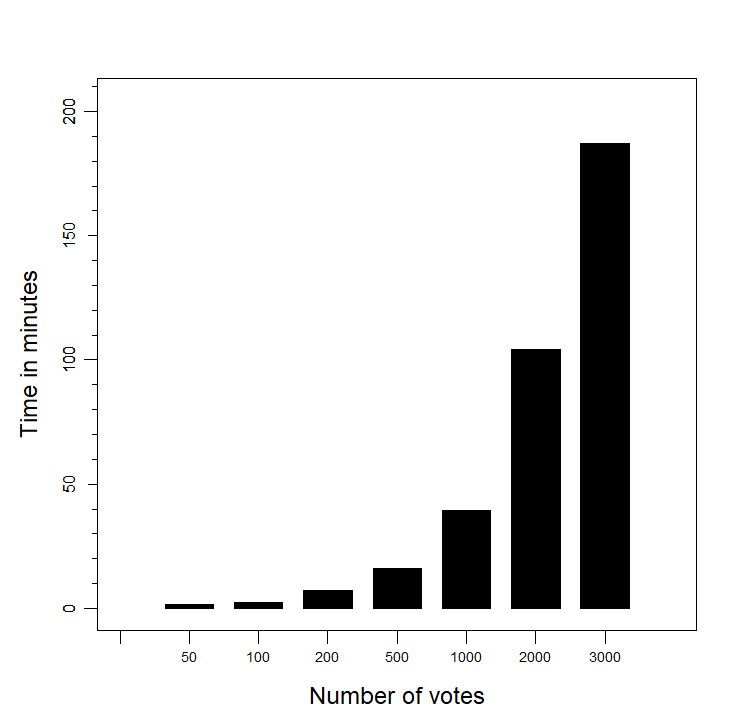
\includegraphics[scale=0.50]{PlotVer3.png}

\end{center}



\section{Analysis}

\noindent\emph{Summary.} The main contribution of our formalisation is that of independently
verifiable \emph{evidence} for a set of candidates to be the winners
of an election counted according to the Schulze method. Our main
claim is that that our notion of evidence is both safeguarding the
privacy of the individual ballot (as the count is based on encrypted
ballots) and is verifiable at the same time (by means of zero
knowledge proofs). To do this, we have axiomatised a set of
cryptographic primitives to deal with encryption, decryption,
correctness of shuffles and correctness of decryption. From formal
and constructive proof of the fact that such evidence can always be
obtained, we have then extracted executable code that is provably
correct by construction and produces election winners together with
evidence once implementations for the cryptographic primitives are
supplied.

In a second step, we have supplied an implementation of these
primitives, largely based on the Unicrypt Library. Our expertiments
have demonstrated that this approach is feasible, but quite clearly
much work is still needed to improve efficiency. 

\smallskip\noindent\emph{Assumptions for Provable Correctness.}
While we claim that the end product embodies a high level of
reliability, our approach necessarily leaves some gaps between the
executable and the formal proofs. First and foremost, this is of
course the implementation of the cryptographic primitives in an
external (and unverified) library. We have minimised this gap by
basing our implementation on a purpose-specific existing library
(Unicrypt) to which we relegate most of the functionality. Another
gap is the extraction mechanism of the Coq theorem prover which does
not come with formal correctness guarantees that reach down to the
machine code level such as for example CakeML~\cite{Kumar:2014:CVI}.

\smallskip\noindent\emph{Modelling Assumptions.} In our modelling of
the cryptographic primitives, in particular the zero knowledge
proofs, we have assumed that zero knowledge proofs can be verified,
whereas in reality zero-knowledge proofs just confirm facts with
very high probability which we have deliberately  ignored. As a
consequence our correctness assertions only hold to the level
of probability that is guaranteed by zero knowledge proofs.

\smallskip\noindent\emph{Scalability.} We have analysed the
feasibility of the extracted code by counting an increasing number
of ballots. While this demonstrates a proof of concept, our results
show that the cryptographic layer adds significant overhead compared
to plaintext tallying \cite{Pattinson:2017:SVE}.  Our present
hypothesis is that this overhead is created by the various layers of
bindings between the executable (extracted into OCaml) and the
Unicrypt library (implemented in Java) as each appears to be very
efficient individually. 

\smallskip\noindent\emph{Future Work.} Our axiomatisation of the
needed cryptographic primitives lays the foundation of creating a
verified library. For scalability, a more detailed analysis (and
profiling) of the software artefact are necessary. Orthogonal to
what we have presented here, it would also be of interest to develop
a provably correct verifier for the notion of certificate presented
here. 

\bibliographystyle{plain}
\bibliography{all2,delta2}

%\appendix
%\section{Discussion and Further Work}
%
%One aspect that we have not considered here is encryption of
%ballots to safe-guard voter privacy which can be incorporated using
%protocols such as shuffle-sum \cite{Benaloh:2009:SSC} and
%homomorphic encryption \cite{Yi:2014:HEA}. The key idea here is to
%formalise a given voting scheme based on encrypted ballots, and then
%to establish a homomorphic property: the decryption of the result
%obtained from encrypted ballots is the same as the result obtained from
%the decrypted ballots.  We leave this to further work.

%\bibliographystyle{myplain}
%\bibliography{all2,delta2}


\end{document}
